\subsection{Full-Wave Bridge-Network Rectifier:}

The {\bfseries\itshape full-wave bridge-network rectifier}, converts alternating current (AC), which periodically reverses direction, to direct current (DC). This type of rectifier, unlike the {\bfseries\itshape half-wave}, during the negative period, reverse the roles of the diodes but maintaining the same polarity for the voltage across the load resistor. Unlike the {\bfseries\itshape center-taped rectifier} that use one diode per semi-period, this network uses two diodes per semi-period. As result we have no lost of voltage. \hfill \break 

Using the 100$\Omega$ resistor as $R_{L}$ and four 1N4003 diodes, the circuit of the Figure 3.6.0 was assembled. 

\begin{figure}[H]
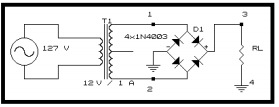
\includegraphics[scale=1]{fwbn.png}
\centering \linebreak \linebreak Figure 3.6.0: Full-wave bridge-network rectifier.
\end{figure}

For measure the signal before being rectified, we put the positive terminal of the voltmeter in the terminal 1 of the Figure 3.6.0 and the negative terminal of the voltmeter in the terminal 3 of the Figure 3.6.0. We will call this voltage $V_{T}$ (Transformer Voltage).

\begin{ceqn}
\begin{align}
V_{T} = 13.35\ V_{rms}
\end{align}
\end{ceqn}

{\bfseries\itshape\color{OliveGreen}{Observation:}} {\bfseries\itshape\color{OliveGreen}{To measure $V_{T}$ the Voltmeter needs to be in the A.C option.}} \hfill \break

In the same terminals ( 1 and 3 ), of the Figure 3.6.0, the terminals of the oscilloscope were connected same as the voltmeter. Now, as can we see in Figure 3.6.1, the signal isn't being rectified yet. To visualize the rectified signal, the terminals of the oscilloscope were connected to the terminals 2 and 3 of the Figure 3.6.0. Now, as we can see in Figure 3.6.2 the signal is rectified from A.C to D.C. Now there's no negative voltage.

\begin{multicols}{2}
\begin{figure}[H]
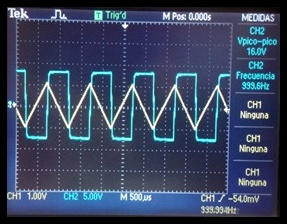
\includegraphics[scale=.48]{o7.jpg}
\centering \linebreak \linebreak Figure 3.6.1: Transformer output signal.
\linebreak \linebreak $\frac{5 V}{div}\ \ and\ \ \frac{5mseg}{div}$.
\end{figure}

\begin{figure}[H]
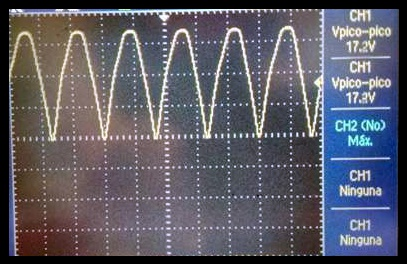
\includegraphics[scale=.54]{o8.jpg}
\centering \linebreak \linebreak Figure 3.6.2: Full-wave rectified signal.
\linebreak \linebreak $\frac{5 V}{div}\ \ and\ \ \frac{5mseg}{div}$.
\end{figure}
\end{multicols}

{\bfseries\itshape\color{OliveGreen}{Observation:}} {\bfseries\itshape\color{OliveGreen}{In the oscilloscope we are only using the channel 1 in D.C option.}}  \hfill \break

To measure the voltage in {\bfseries\itshape $R_{L}$}, its necessary to connect the positive terminal of the voltmeter in the terminal 2 of the Figure 3.6.0 and the negative terminal of the voltmeter in the terminal 3 of the Figure 3.6.0. We will call this voltage $V_{0}$, also the resistor $R_{L}$ will have a current, we will call it $I_{0}$ and with Ohm's Law we can find it.

\begin{ceqn}
\begin{align}
V_{0} = 10.4\ V_{rms} 
\end{align}
\end{ceqn} \hfill

{\bfseries\itshape\color{OliveGreen}{Observation:}} {\bfseries\itshape\color{OliveGreen}{To measure $V_{0}$ the Voltmeter needs to be in the D.C option.}} \hfill \break \break

{\bfseries\itshape\color{Maroon}{Using Ohm's Law: $I = \frac{V_{0}}{R_{L}}.$}} \hfill \break

\begin{ceqn}
\begin{align}
I_{0} = \frac{10.4\ V_{rms}}{0.100\ \Omega} = 0.104\ A
\end{align}
\end{ceqn} \hfill 

{\bfseries\itshape
\begin{itemize}
\item For $V_{p}$ ( Peak Voltage ) of Figure 3.6.1:
\end{itemize}} 

When the terminals of the oscilloscope are connected to the circuit and the signal it's displayed on screen as Figures 3.6.1 shows. We will put the oscilloscope in the option {\bfseries\itshape measures} and search for the option {\bfseries\itshape Max Voltage}. \hfill \break

\begin{ceqn}
\begin{align}
V_{p} = 18.6 V
\end{align}
\end{ceqn} \hfill 

{\bfseries\itshape
\begin{itemize}
\item Finally, $V_{p} - V_{D}$, where $V_{p}$ it's the peak voltage in Figure 3.6.1 and $V_{D}$ it's the diode Voltage:
\end{itemize}} \hfill

\begin{ceqn}
\begin{align}
V_{p} - ( 2 )V_{D} = 18.6 V - ( 2 )( 0.7 V ) = 17.2 V
\end{align}
\end{ceqn}

\pagebreak